\subsection{Cauchy's Theorem}
The previous proposition tells us that $\omega$ has a primitive if and only if its integral over every (piecewise $C^1$) closed curve is 0. This is a somewhat difficult condition to work with. However, if we are working in a disk, we can check a much simpler condition. In a disk, a form $\omega$ has a primitive if and only if its integral over the boundary of every rectangle (one whose sides are parallel to the axes) is 0. This is simply because in a disk we can connect any two points with a path that travels parallel to the axes. Thus although it might be difficult to determine whether a form has a primitive or not, doing this locally is not too hard. This motivates the following definition.

\begin{definition}[Closed forms]
A form $\omega$ is \textit{closed} if it locally has a primitive.
\end{definition}
\begin{remark}
We will check soon that this definition of closed agrees with the usual definition of $d\omega = 0$.
\end{remark}
By the prior discussion, it is easy to see that a form $\omega$ is closed if and only if the integral over the boundary of sufficiently small rectangles is 0. If the form locally has a primitive, then given a point there is a neighbourhood within which the form has a primitive and hence the integral rectangle boundaries contained in this neighbourhood is 0. On the other hand, if the integral over the boundaries of sufficiently small rectangles is 0, we can define primitives on disks containing these rectangles. In fact by noting that any rectangle can subdivided into a number of arbitrarily small rectangles, we can say that a form is closed if and only the integral over the boundary of \textit{any} rectangle is 0.

It is important to note that the existence of a local primitives does not necessarily imply the existence of a global primitive (although we know in some cases it does such as in disks). As an example, consider $\Omega = \C \setminus \{0\}$ and the form
$$ \omega = \frac{dz}{z}$$
We know $\omega$ is closed because locally at every point of $\Omega$ there's a branch of $\log z$, which forms a local primitives for $\omega$. However we claim that there is no global primitive. In order to verify this, it is enough to find a closed curve $\gamma$ on which $\int_\gamma \omega \neq 0$. We will take $\gamma = e^{it}$ for $t \in [0, 2\pi]$. Since $z = e^{it}$ we have $dz = ie^{it} dt$. Therefore
\begin{align*}
    \int_{\gamma} \frac{dz}{z} = \int_{0}^{2\pi} \frac{ie^{it} dt}{e^{it }} = 2\pi i 
\end{align*}
Such an example need not be complex. For example if we write $z = x + iy$ then
$$ \frac{d(x + iy)}{x + iy} = \frac{xdx + ydy}{x^2 + y^2} + i \frac{xdy - ydx}{x^2 + y^2} $$
Without any calculations then, by looking at the complex result, we can conclude that
$$ \int_{\gamma} \underbrace{\frac{xdy - ydx}{x^2 + y^2}}_{\eta} = 2\pi $$
Note that this particular form $\eta$ is equal to $dt$ where $t = \arctan(\frac{y}{x})$

\subsection{\textit{Aside: Green's Theorem}}
Before we move on to proving Cauchy's theorem, let us quickly verify that our definition of closed forms agrees with the usual definition.

Suppose $P, Q$ are continuous with continuous partials $\frac{\partial P}{\partial y}$ and $\frac{\partial Q}{\partial x}$ in a neighbourhood of a closed rectangle $A$. Let $\gamma$ denote the boundary of $A$. Then by Green's Theorem we know that 
$$ \int_\gamma P dx + Qdy = \iint_A \left( \frac{\partial Q}{\partial x} - \frac{\partial P}{\partial y} \right)dxdy $$
We can prove Green's Theorem by simple evaluation.
\begin{align*}
    \iint_A \frac{\partial Q}{\partial x} dx dy &= \int_{b_1}^{b_2} \left( \int_{a_1}^{a_2} \frac{\partial Q}{\partial x} dx \right) dy\\
    &= \int_{b_1}^{b_2} Q(a_2, y) - Q(a_1, y) dy\\
    &= \int_{a_1}^{a_2} Q(x, b_1) dx + \int_{b_1}^{b_2} Q(a_2, y) dy + \int_{a_2}^{a_1} Q(x, b_2) dx + \int_{b_2}^{b_1} Q(a_1, y) dy\\
    &= \int_\gamma Q dy
\end{align*}
where we use the fact that $Q$ is constant on the horizontal sides. Doing a similar calculation with $\frac{\partial P}{\partial y}$ and summing the results, we get Green's Theorem.
\begin{figure}
    \centering
    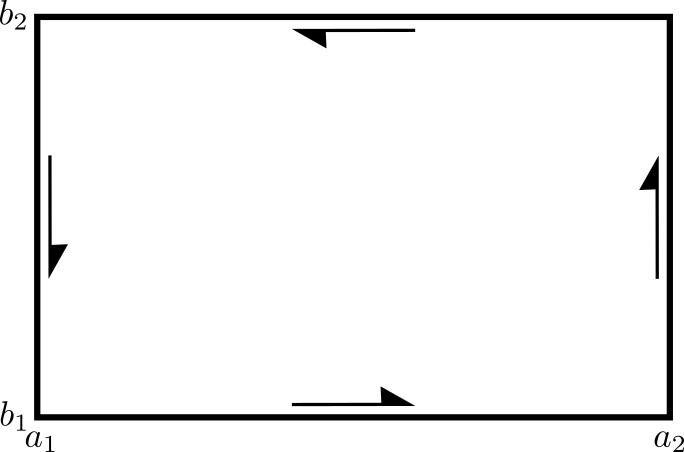
\includegraphics[scale=0.7]{Images/integral_over_rectangle.png}
    \caption{Integrating over the boundary of a rectangle}
    \label{fig:integrate-over-bd-rect}
\end{figure}

Now suppose $\omega = Pdx + Qdy$ is such that its integral over the boundary $\gamma$ of any sufficently small rectangle $A$ is 0. By Green's theorem this happens if and only if
$$ \iint_A \left( \frac{\partial Q}{\partial x} - \frac{\partial P}{\partial y} \right)dxdy = 0 $$
Thus if $d\omega = 0$ then it is obvious that the integral over the boundary of any rectangle is 0.
In order to see the converse, suppose the integral over any small rectangle is 0 then the form must be 0 everywhere (if it was non-zero at some point, it would be non-zero in a neighbourhood and so the integral over a rectangle contained in this neighbourhood would be non-zero). Therefore we conclude
$$ \left( \frac{\partial Q}{\partial x} - \frac{\partial P}{\partial y} \right)dxdy = 0 $$
but that is exactly saying $d\omega = 0$.

\begin{center}
    \rule{2cm}{0.4pt}
\end{center}

Now we can move on to proving Cauchy's Theorem. 
\begin{theorem}[Cauchy's Theorem]\label{thm:cauchy-thm}
If $f(z)$ is holomorphic in an open subset $\Omega \subset \C$ then $f(z)dz$ is closed.
\end{theorem}
We first show a very simple proof in the case where $\frac{\partial f}{\partial x}$ and $\frac{\partial f}{\partial y}$ exist and are continuous. While we don't want to prove the statement with this assumption (in fact we will use Cauchy's theorem to show that the partials of holomorphic functions exist and are continuous), it is interesting to note how short and simple the proof is in this case.
\begin{proof}
We can write
$$ f(z) dz = f(z) d(x + iy) = \underbrace{f(z)}_P dx + \underbrace{if(z)}_Q dy $$
By Green's formula, in order to show $f$ is closed, it suffices to show that
$$ \frac{\partial P}{\partial y} = \frac{\partial Q}{\partial x} $$
Substituting the actual values of $P$ and $Q$ into this statement, we see we want to show that
$$ \frac{\partial f}{\partial y} = i \frac{\partial f}{\partial x} $$
But this is exactly what it means to be holomorphic. 
\end{proof}

A lovely proof that we cannot use. Instead we have the following.
\begin{proof}
In order to show $f$ is closed we know it is sufficient to show that 
$$ \int_\gamma f(z) dz = 0 $$
where $\gamma$ is the boundary of any rectangle $R$ in $\Omega$. Let us call the value of the integral $\mu(R)$. Suppose we divide $R$ into 4 equal parts $R_i$ each with oriented boundary $\gamma_i$. Then
$$ \int_\gamma f(z) dz = \sum_{i = 1}^4 \int_{\gamma_i} f(z) dz $$
Then there is at least one $i$ such that
$$ \abs{ \int_{\gamma_i} f(z) dz } \geq \frac{1}{4} \abs{ \int_\gamma f(z) dz } $$
Let us define $R_i := R^{(1)}$ and $\gamma_i := \gamma^{(1)}$. From here we can repeatedly apply this procedure to obtain a chain of rectangles $R \supset R^{(1)} \supset R^{(2)} \subset \dots$. Then
\begin{equation}\label{eq:cauchy-thm-ineq-1}
    \abs{\mu(R^{(k)}} = \abs{\int_{\gamma^{(k)}} f(z) dz} \geq  \frac{1}{4^k} \abs{ \int_\gamma f(z) dz } = \frac{1}{4^k} \abs{\mu(R)}
\end{equation}
\begin{figure}[ht]
    \centering
    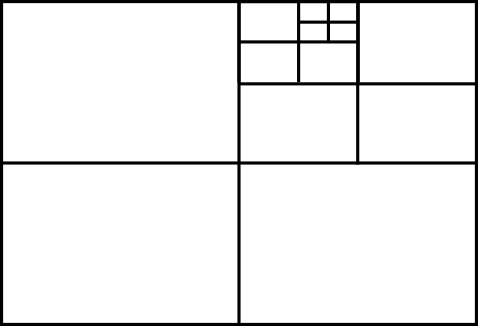
\includegraphics{Images/cauchy_thm_division.png}
    \caption{Divide $R$ into a chain of rectangles}
    \label{fig:cauchy-thm-div}
\end{figure}

Note there exists a (unique) point $z_0$ in $\bigcap_{k = 1}^\infty R^{(k)}$ (this is one of the characterisations of compact sets). Since $f$ is holomorphic at $z_0$ we can write
$$ f(z) = f(z_0) + f'(z_0)(z - z_0) + \phi(z)\abs{z - z_0} $$
where $\phi(z) \to 0$ as $z \to 0$. In particular this means that given any $\epsilon > 0$, there exists some $\delta > 0$ so that $\abs{z - z_0} < \delta$ implies that $\abs{\phi(z)} < \epsilon$. Then
$$ \int_{\gamma^{(k)}} f(z) dz = \int_{\gamma^{(k)}} f(z_0) dz + \int_{\gamma^{(k)}} f'(z_0)(z - z_0) dz + \int_{\gamma^{(k)}} \phi(z)\abs{z - z_0} dz $$
The first two terms are 0 since both forms have primitives ($f(z_0)z$ and $\frac{f'(z_0)}{2}(z - z_0)^2$ respectively) which are being integrated over a closed curve. What we want to show then is that the last term is also 0. Suppose we take $k$ sufficiently large so that $\abs{z - z_0} < \delta$ for all $z \in R^{(k)}$. Then
$$ \abs{\int_{\gamma^{(k)}} \phi(z) \abs{z - z_0} dz} \leq \epsilon \int_{\gamma^{(k)}} \abs{z - z_0} dz \leq \epsilon \text{ diam}(R^{(k)}) \text{ perm}(R^{(k)})$$
where $\text{diam}(R^{(k)})$ is the maximum distance between two points in $R^{(k)}$ and $\text{perm}(R^{(k)})$ is the perimeter of the rectangle. Both these quantities half as we iterate implying that 
$$\abs{\int_{\gamma^{(k)}} f(z) dz} \leq \frac{1}{4^k} \epsilon \text{ diam}(R) \text{ perm}(R)$$
Then by \eqref{eq:cauchy-thm-ineq-1} we conclude
\begin{align*}
    \abs{\mu(R)} \leq 4^k \abs{ \int_{\gamma^{(k)}} f(z) dz } \leq \epsilon \text{ diam}(R) \text{ perm}(R)
\end{align*}
Since $\epsilon$ was arbitrary, we conclude that $\abs{\mu(R)} = 0$. 
\end{proof}

\begin{corollary}
Holomorphic functions $f(z)$ in open $\Omega \subset \C$ locally have a primitive which is holomorphic.
\end{corollary}
\begin{proof}
By Cauchy's Theorem we know that holomorphic functions in open subsets of $\C$ are closed. This is equivalent to saying that they have a local primitive. Let $F$ be such a local primitive for $f$. This means that
$$ f(z)dz = dF = \frac{\partial F}{\partial z}dz + \frac{\partial F}{\partial \ol{z}} d\ol{z} $$
in some neighbourhood.
Recall that $dz$ and $d\ol{z}$ are linearly independent. Then since the coefficient of $d\ol{z}$ is 0 on the left hand side, it must also be 0 on the right hand 0 implying that
$$ \frac{\partial F}{\partial \ol{z}} = 0 $$
which is one of the (many) equivalent formulations for being holomorphic.
\end{proof}

\begin{corollary}\label{cor:cauchy-thm-general}
Cauchy's Theorem remains true if $f(z)$ is continuous in $\Omega$ and holomorphic everywhere except possibly on a line. In particular then a continuous function that is holomorphic except on a finite number of points is holomorphic everywhere.
\end{corollary}
\begin{proof}
    We assume that the line on which $f$ is not holomorphic is parallel to real axis since other cases are quite similar. 
    We want to show that the integral over the boundary of a rectangle is still 0. If the rectangle does not intersect the line at all, we are done. The other possibilities are the line intersects the boundary at two points or the line 
    goes through an edge. 

    Let us consider the latter case first. In this case, we can take another rectangle whose edge is $\epsilon$ away from the original rectangle, as shown in \autoref{fig:cauchy-thm-gen}. 
    \begin{figure}[ht]
        \centering
        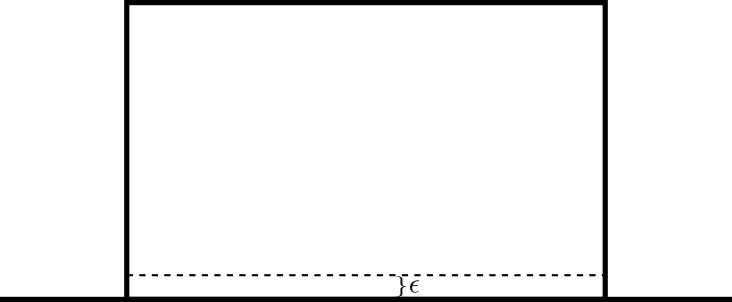
\includegraphics{Images/cauchy_thm_gen.png}
        \caption{Rectangle with non-holomorphic edge}
        \label{fig:cauchy-thm-gen}
    \end{figure}
    We know the integral over the boundary of the smaller rectangle is 0 for every $\epsilon > 0$ and as we let $\epsilon \to 0$, the integral converges to the integral over the boundary of the desired rectangle which therefore must be 0. of the If we are instead in a situation like \autoref{fig:cauchy-thm-gen2}, then we can reduce it back to the prior case by integrating on the upper and lower halves separately and summing the values.
    \begin{figure}[ht]
        \centering
        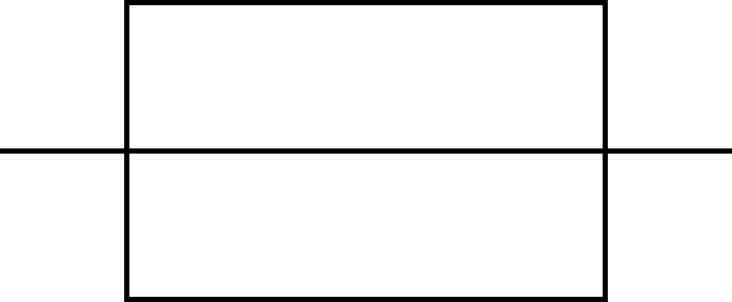
\includegraphics{Images/cauchy_thm_gen2.png}
        \caption{Rectangle intersecting non-holomorphic edge}
        \label{fig:cauchy-thm-gen2}
    \end{figure}
\end{proof}
\begin{remark}
    It is important the function be continuous everywhere. For example, $f(z) = \frac{1}{z}$ is holomorphic everywhere except the origin so one might expect there to be a holomorphic extension of $f$ on all of $\C$ based on the previous proposition. But in fact the proposition does not apply since $f$ is not continuous at 0 (and indeed there is no holomorphic extension of $f$ onto $\C$. We will be able to prove this quite easily with the tools discussed later). 

    Where the proof breaks down in the discontinuous case is in our assumption that as $\epsilon \to 0$, we have a convergence of the integrals. Obviously this can only hold true if we have some control over how much $f$ can vary in small neighbourhoods.
\end{remark}

\section{Cauchy's Integral Formula}

\subsection{Primitives along curves}
In general a closed differential form $\omega$ in an open set $\Omega$ need not have a primitive. However, we can always find what is called a \textit{primitive along a curve}. We know that closed forms always have local primitives. So a primitive along a curve is simply a continuous function that agrees with all the local primitives along the curve. This definition is made precise in the following proposition.

\begin{proposition}\label{prop:primitive-along-curve}
Let $\Omega \subset \C$ be open and let $\omega$ be a closed form in $\Omega$. Also suppose $\gamma: [a, b] \to \Omega$ is a continuous curve. Then there is a continuous functions $f(t)$ on $[a, b]$ such that for every $t_0 \in [a, b]$ there is a local primitive $F$ of $\omega$ in a neighbourhood of $\gamma(t_0)$ such that 
$$ f(t) = F(\gamma(t)) $$
for all $t$ in some neighbourhood of $t_0$. Moreover, $f$ is uniquely determined up to the addition of a constant.
\end{proposition}
\begin{proof}
    The uniqueness is easy to determine. Suppose $f_1, f_2$ are primitives of $\omega$ along $\gamma$. Then in a neighbourhood of $t_0$ we have
    $$ f_1(t) - f_2(t) = F_1(\gamma(t)) - F_2(\gamma(t)) $$
    where $F_1, F_2$ are two local primitives of $\omega$. Since they are primitives we know they can only differ by a constant. But this means that $f_1(t) - f_2(t)$ is only constant on some neighbourhood of $t_0$. This means $f_1 - f_2$ is locally constant but since $[a, b]$ is connected we conclude that $f_1 - f_2$ is constant everywhere.
    
    The slightly trickier thing to do is show existence of $f$. We would like to define $f$ at a point to be simply be the value of the local primitive at that point. The problem is that a point might lie in the neighbourhood for two different primitives. Therefore what we will do is split the curve into a different parts where we have a primitive on each of the smaller parts and just show we can get agreement on the intersections. 

    \begin{figure}
        \centering
        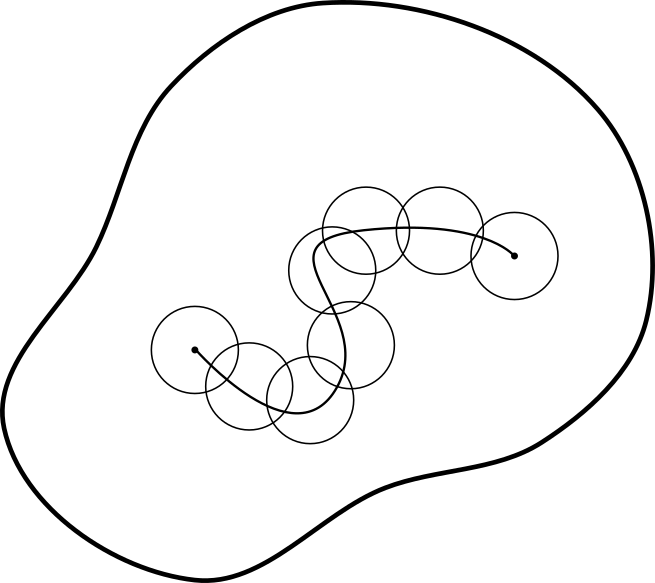
\includegraphics[scale=0.7]{Images/primitives_along_curves.png}
        \caption{Local primitives are defined on each disk, just need to make them agree on the intersection}
        \label{fig:prim-along-curve}
    \end{figure}
    
    So first we find a partition $a = t_0 < t_1 < \dots < t_n = b$ of the interval so that  every $\gamma([t_{i - 1}, t_i])$ lies in an open disk $U_i$ in which $\omega_i$ has a primitive $F_i$ (the Lebesgue number lemma guarantees the existence of such a partition). Since the $U_i$ are disks their intersection (if non-empty) is connected. This means that $F_i - F_{i - 1}$ is constant on $U_i \cap U_{i - 1}$ (again, primitives can only differ by a constant). Thus we simply adjust these constants one at a time for $i = 1, \dots, n$ so that we have agreement on all the intersections. Finally, we define $f(t) = F_i(\gamma(t))$ where $t \in [t_{i - 1}, t_i]$.
\end{proof}

The primitive along a curve behaves at least somewhat like a genuine primitive. For example, we have the following.

\begin{corollary}
Suppose $\gamma: [a, b] \to \Omega$ is a piecewise $C^1$ curve and $f$ is a primitive along $\gamma$. Then
$$ \int_\gamma \omega = f(b) - f(a) $$
\end{corollary}
\begin{proof}
    Using notation as in the previous proposition, define $\gamma_i := \gamma|_{[t_{i - 1}, t_i]}$. Then
    \begin{align*}
       \int_\gamma \omega &= \sum_{i = 1}^n \int_{\gamma_i} \omega \\
       &= \sum_{i = 1}^n F_i(\gamma(t_i)) - F_i(\gamma(t_{i - 1}))\\
       &= \sum_{i = 1}^n f(t_{i}) - f(t_{i - 1})\\
       &= f(b) - f(a)
    \end{align*}
\end{proof}
Note that for the statement although the left-hand side requires $\gamma$ to be $C^1$ the right-hand side makes even if $\gamma$ is just continuous (we only needed continuity of $\gamma$ in \autoref{prop:primitive-along-curve}). This allows us to define
$$ \int_\gamma \omega $$
even for continuous curves as $f(b) - f(a)$ where $f$ is simply a primitive along $\gamma$ (since primitives along curves only differ by a constant this is well-defined).

We can use this idea to get some very nice things very easily. For example suppose $\gamma$ is a closed curve not containing 0. Then
$$ \int_{\gamma} \frac{1}{z}dz = f(b) - f(a) $$
where, as usual, $f$ is a primitive along $\gamma$. But we know that a primitive of $\frac{1}{z}dz$ is $\log$ so $f(b) - f(a)$ is the difference between two branches of $\log$ at $\gamma(a) = \gamma(b)$. Therefore we know that $f(b) - f(a) = 2\pi i n$ where $n$ is some integer. Similarly we can conclude that
$$ \int_\gamma \frac{xdy - ydx}{x^2 + y^2} = 2\pi n $$
(for the same $n$). One can see that it measures how the argument of $z$ changes along $\gamma$. Thus we often call the integral on the left the ``variation of $\arg(z)$ along $\gamma$''.

\subsection{Homotopy}
Homotopy roughly talks about transforming one curve to another in some kind of continuous manner. In fact, we discuss two flavours of it depending on whether the curves share endpoints or whether they are closed curves.

\begin{definition}[Homotopy of curves with fixed endpoints]
Suppose $\gamma_0, \gamma_1: [0, 1] \to \Omega$ be continuous curves with the same endpoints (i.e. $\gamma_0(0) = \gamma_1(0)$ and $\gamma_0(1) = \gamma_1(1)$). Then $\gamma_0$ and $\gamma_1$ are said to be \textit{homotopic} (with fixed endpoints) if there is a continuous function $\gamma: [0, 1] \times [0, 1] \to \Omega$ such that
\begin{align*}
    \gamma(0, t) &= \gamma_0(t)\\
    \gamma(1, t) &= \gamma_1(t)\\
    \gamma(s, 0) &= \gamma_0(0) = \gamma_1(0)\\
    \gamma(s, 1) &= \gamma_0(1) = \gamma_1(1)
\end{align*}
\end{definition}
\begin{figure}[ht]
    \centering
    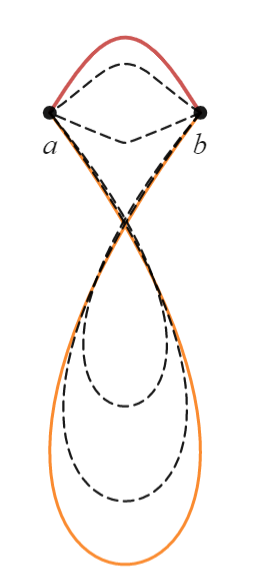
\includegraphics[scale=0.8]{Images/homotopy_example.png}
    \caption{Homotopic curves with fixed endpoints. Dotted lines indicates the homotopy between the two curves (see \href{https://www.desmos.com/calculator/jsdrzz6v0d}{desmos} for interactive version).}
    \label{fig:homotopic-fixed-ends}
\end{figure}

\begin{definition}[Homotopy of closed curves]
Suppose $\gamma_0, \gamma_1: [0, 1] \to \Omega$ be closed curves (i.e. $\gamma_0(0) = \gamma_0(1)$ and $\gamma_1(0) = \gamma_1(1)$ but it need not be true that $\gamma_0(0) = \gamma_1(0)$). Then $\gamma_0$ and $\gamma_1$ are said to be \textit{homotopic} (as closed curved) if there is a continuous function $\gamma: [0, 1] \times [0, 1] \to \Omega$ such that for every $s, t \in [0, 1]$ we have
\begin{align*}
    \gamma(0, t) &= \gamma_0(t)\\
    \gamma(1, t) &= \gamma_1(t)\\
    \gamma(s, 0) &= \gamma(s, 1)
\end{align*}
We say $\gamma_0$ is homotopic to a point or \textit{nullhomotopic} if $\gamma_1$ is a constant map.
\end{definition}
\begin{figure}
    \centering
    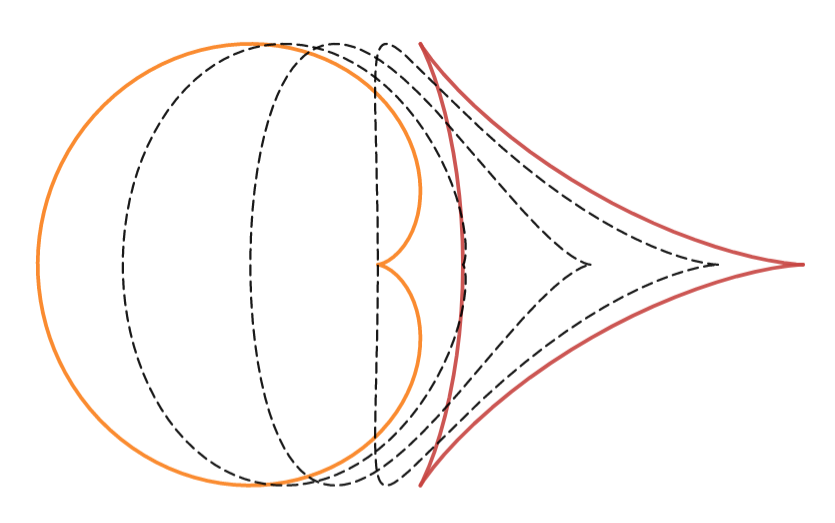
\includegraphics[scale=0.7]{Images/homotopy_example_closed_curves.png}
    \caption{Homotopic closed curves. Dotted lines indicate homotopy between the curves (see \href{https://www.desmos.com/calculator/ihxwimjylv}{desmos} for interactive version).}
    \label{fig:homotopic-closed-curves}
\end{figure}

See \autoref{fig:homotopic-fixed-ends} and \autoref{fig:homotopic-closed-curves} for examples of the two kinds of homotopies.\\


